\section{Data Models}\label{sec:dataModels}
Given the Tycho2 catalog of stars, how can we model our data our data for efficient spatial queries?

\subsection{Relational Data Model}\label{subsec:relationalDataModel}
The relational data model is the most popular data abstraction, and arguably the most natural.
Here data is stored in tuples.
The schema is defined before data is added, meaning that each tuple of a given table has the same number of attributes.
If thought of as a table, the number of columns is fixed by the number of tuples is variable.
Interaction between this model involves the use of relational algebra.

In terms of distributed relational DBMSs, most implementations are consistent, available but not partition tolerant.

\subsection{Column Family Data Model}\label{subsec:columnFamilyDataModel}
\begin{figure}
    \centering{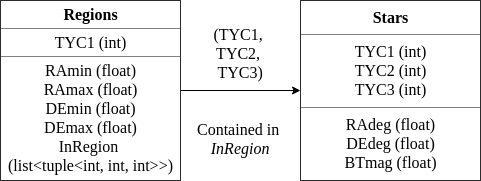
\includegraphics[scale=0.5]{images/cassandra-data-model.png}}
    \caption{Depiction of data model used with Cassandra.
    There exists a \textit{Stars} column family indexed by \texttt{TYC1, TYC2, TYC3}, and a \textit{Regions} column
    family indexed by \texttt{TYC1}.
    The \textit{Regions} family has a list of \texttt{TYC} IDs of stars contained in that region.}
    \label{fig:cassandraDataModel}
\end{figure}

The column family data model can be loosely thought of as the segmentation of a relational table into several two
column tables consisting of a single attribute of the original table and a primary key based off this attribute.
These segmented tables can then be grouped into a column family, which represents a group of columns indexed by the
same primary key.
This segmentation is useful for allowing denormalization, meaning that the schema does not have to be defined before
data insertion and that each primary key does not have to map the same amount of columns as other keys.
Column family models are known for this denormalization and efficient querying, accessing only the columns required for
the query itself.

\textit{Apache Cassandra} is the column store database that is being tested here, and is a form of a
\textit{distributed} DBMS\@.
Cassandra itself is available and partition tolerant, but not consistent.
Data in a Cassandra cluster is hash partitioned by the primary key, and these pieces can be replicated across the
cluster as well.

The data model being implemented with Cassandra involves two column families: \textit{Regions} and \textit{Stars}.
The \textit{Stars} family has six columns:
\begin{multicols}{3}
    \begin{itemize}
        \item[] \texttt{TYC1}
        \item[] \texttt{TYC2}
        \item[] \texttt{TYC3}
        \item[] \texttt{RAmdeg}
        \item[] \texttt{DEmdeg}
        \item[] \texttt{BTmag}
    \end{itemize}
\end{multicols}
where the first three columns represent the star's ID, \texttt{RAmdeg, DEmdeg} represent the star's position, and
\texttt{BTmag} represents the magnitude of the star.
This is depicted in~\autoref{fig:cassandraDataModel}.
The primary key for this family is the GSC region \texttt{TYC1}, with \texttt{TYC2, TYC3} as secondary clustering
keys.
Efficient queries for stars should involve the primary key \texttt{TYC1}.

The \textit{Regions} family has six columns as well:
\begin{multicols}{3}
    \begin{itemize}
        \item[] \texttt{TYC1}
        \item[] \texttt{RAmin}
        \item[] \texttt{RAmax}
        \item[] \texttt{DEmin}
        \item[] \texttt{DEmax}
        \item[] \texttt{InRegion}
    \end{itemize}
\end{multicols}
where \texttt{TYC1} represents the region ID, \texttt{RAmin, RAmax} represent the right ascension limits,
\texttt{DEmin, DEmax} represent the declination limits, and \texttt{InRegion} is a list of star IDs contained within
that region.
Each region's primary key is the \textit{TYC1} region ID, and it follows that efficient region queries will use only
the primary key.

%To query for all attributes of stars within a region, we first query for the \texttt{InRegion} column in the
%\textit{Region} family given the \texttt{TYC1}.
%Every star returned from this query is then used to search all columns of the \textit{Stars} family.

\subsection{Graph Data Model}\label{subsec:graphDataModel}
\begin{figure}
    \centering{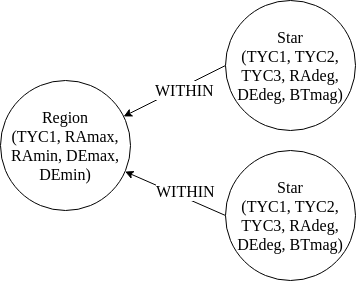
\includegraphics[scale=0.5]{images/neo4j-data-model.png}}
    \caption{Depiction of data model used with Neo4J.
    There exists a collection of \textit{Star} nodes and \textit{Region} nodes, each of which are related by the
    \texttt{WITHIN} relationship.}
\end{figure}

Relative to the relational data model, the graph data model focuses on the relationship between various tuples.
Here data is stored in nodes as attributes, and relationships are stored as edges between nodes.
Data is accessed by simply traversing the graph.
Graph models shine in relationship querying and denormalization as opposed to a relational data model.

\textit{Neo4J} is the graph database that is being tested here, and is also a form of a distributed DBMS\@.
The Neo4J setup that was tested here is available and consistent (like typical RDBMS), but not partition tolerant.
Data in a Neo4J cannot be partitioned like Cassandra, meaning that every node is a full replica.

The data model being implemented here involves two types of nodes: \textit{Region} and \textit{Star} nodes.
A \textit{Star} node has the same attributes as the columns in the Cassandra \textit{Stars} column family.
\textit{Regions} have all attributes in the columns of the \textit{Regions} column family except for the
\texttt{InRegion} column.
Instead, a \texttt{WITHIN} relationship is established between all \textit{Star} nodes that exist in Region.

%To query for all attributes for a star within a region, we first search for the \textit{Region} node that matches
%some \texttt{TYC1} ID\@.
%The next step involves traversing all \texttt{WITHIN} edges to each \textit{Star} node and returning the attributes.